%\documentclass[a4paper,11pt]{book}
\documentclass[a4paper,twoside,11pt,titlepage]{book}
\usepackage{listings}
\usepackage[utf8]{inputenc}
\usepackage[spanish]{babel}

\usepackage{xspace}

% \usepackage[style=list, number=none]{glossary} %
%\usepackage{titlesec}
%\usepackage{pailatino}

\decimalpoint
\usepackage{dcolumn}
\newcolumntype{.}{D{.}{\esperiod}{-1}}
\makeatletter
\addto\shorthandsspanish{\let\esperiod\es@period@code}
\makeatother


%\usepackage[chapter]{algorithm}
\RequirePackage{verbatim}
%\RequirePackage[Glenn]{fncychap}
\usepackage{fancyhdr}
\usepackage{graphicx}
\usepackage{afterpage}
\usepackage{longtable}
\usepackage{natbib}
\usepackage{float}


% ********************************************************************
% Re-usable information
% ********************************************************************
\newcommand{\myTitle}{FPGAs de Xilinx \xspace}
\newcommand{\mySubTitle}{Plataforma didáctica para desarrollo de sistemas basados en FPGAs de Xilinx}
\newcommand{\myDegree}{Grado en Ingeniería Informática\xspace}
\newcommand{\myName}{Elena Cantero Molina (alumna)\xspace}
\newcommand{\myProf}{María Begoña del Pino Prieto (tutora)\xspace}
%\newcommand{\mySupervisor}{Put name here\xspace}
\newcommand{\myFaculty}{Escuela Técnica Superior de Ingenierías Informática y de Telecomunicación\xspace}
\newcommand{\myFacultyShort}{E.T.S. de Ingenierías Informática y de
Telecomunicación\xspace}
%\newcommand{\myDepartment}{Departamento de ...\xspace}
\newcommand{\myUni}{\protect{Universidad de Granada}\xspace}
\newcommand{\myLocation}{Granada\xspace}
\newcommand{\myTime}{\today\xspace}
\newcommand{\myVersion}{Version 0.1\xspace}

\usepackage{url}
\usepackage{colortbl,longtable}
\usepackage[stable]{footmisc}
%\usepackage{index}

\pagestyle{fancy}
\fancyhf{}
\fancyhead[LO]{\leftmark}
\fancyhead[RE]{\rightmark}
\fancyhead[RO,LE]{\textbf{\thepage}}
\renewcommand{\chaptermark}[1]{\markboth{\textbf{#1}}{}}
\renewcommand{\sectionmark}[1]{\markright{\textbf{\thesection. #1}}}

\setlength{\headheight}{1.5\headheight}

\newcommand{\HRule}{\rule{\linewidth}{0.5mm}}

\definecolor{gray97}{gray}{.97}
\definecolor{gray75}{gray}{.75}
\definecolor{gray45}{gray}{.45}
\definecolor{gray30}{gray}{.94}

\lstset{ frame=Ltb,
     framerule=0.5pt,
     aboveskip=0.5cm,
     framextopmargin=3pt,
     framexbottommargin=3pt,
     framexleftmargin=0.1cm,
     framesep=0pt,
     rulesep=.4pt,
     backgroundcolor=\color{gray97},
     rulesepcolor=\color{black},
     %
     stringstyle=\ttfamily,
     showstringspaces = false,
     basicstyle=\scriptsize\ttfamily,
     commentstyle=\color{gray45},
     keywordstyle=\bfseries,
     %
     numbers=left,
     numbersep=6pt,
     numberstyle=\tiny,
     numberfirstline = false,
     breaklines=true,
   }
 
% minimizar fragmentado de listados
\lstnewenvironment{listing}[1][]
   {\lstset{#1}\pagebreak[0]}{\pagebreak[0]}

 
\lstdefinestyle{Consola}
   {basicstyle=\scriptsize\bf\ttfamily,
    backgroundcolor=\color{gray30},
    frame=single,
    numbers=none
   }


\newcommand{\bigrule}{\titlerule[0.5mm]}


%Para conseguir que en las páginas en blanco no ponga cabecerass
\makeatletter
\def\clearpage{%
  \ifvmode
    \ifnum \@dbltopnum =\m@ne
      \ifdim \pagetotal <\topskip
        \hbox{}
      \fi
    \fi
  \fi
  \newpage
  \thispagestyle{empty}
  \write\m@ne{}
  \vbox{}
  \penalty -\@Mi
}
\makeatother

\usepackage{pdfpages}
\begin{document}
\begin{titlepage}
 
 
\newlength{\centeroffset}
\setlength{\centeroffset}{-0.5\oddsidemargin}
\addtolength{\centeroffset}{0.5\evensidemargin}
\thispagestyle{empty}

\noindent\hspace*{\centeroffset}\begin{minipage}{\textwidth}

\centering

\includegraphics[width=0.9\textwidth]{imagenes/logo_ugr.jpg}\\[1.4cm]

\textsc{ \Large TRABAJO FIN DE GRADO\\[0.2cm]}
\textsc{ INGENIERÍA EN INGENIERÍA INFORMÁTICA}\\[1cm]
% Upper part of the page
% 
% Title
{\Huge\bfseries \myTitle}
\noindent\rule[-1ex]{\textwidth}{3pt}\\[3.5ex]
{\large\bfseries \mySubTitle}
\end{minipage}

\vspace{2.5cm}
\noindent\hspace*{\centeroffset}\begin{minipage}{\textwidth}
\centering

\textbf{Autora}\\ {\myName}\\[2.5ex]
\textbf{Directora}\\
{\myProf}\\[2cm]

\includegraphics[width=0.3\textwidth]{imagenes/etsiit_logo.png}\\[0.1cm]
\textsc{\myFaculty}\\
\textsc{---}\\
\textsc{\myLocation, \myTime}
\end{minipage}
%\addtolength{\textwidth}{\centeroffset}
%\vspace{\stretch{2}}
\end{titlepage}



%%\thispagestyle{empty}
%\cleardoublepage

\thispagestyle{empty}

\begin{center}
{\large\bfseries Título del Proyecto: \mySubTitle}\\
\end{center}
\begin{center}
\myName\\
\end{center}

Introducción y/o presentación

%\vspace{0.7cm}
\noindent{\textbf{Palabras clave}: palabra\_clave1, palabra\_clave2, palabra\_clave3, ......}\\

\vspace{0.7cm}
\noindent{\textbf{Resumen}}\\

Poner aquí el resumen.
\cleardoublepage


\thispagestyle{empty}


\begin{center}
{\large\bfseries Project Title: Project Subtitle}\\
\end{center}
\begin{center}
First name, Family name (student)\\
\end{center}

%\vspace{0.7cm}
\noindent{\textbf{Keywords}: Keyword1, Keyword2, Keyword3, ....}\\

\vspace{0.7cm}
\noindent{\textbf{Abstract}}\\

Write here the abstract in English.

\clearpage
\thispagestyle{empty}

\noindent\rule[-1ex]{\textwidth}{2pt}\\[4.5ex]

Yo, \textbf{Elena Cantero Molina}, alumna de la titulación \myDegree de la \textbf{Escuela Técnica Superior
de Ingenierías Informática y de Telecomunicación de la Universidad de Granada}, con DNI 45744912M, autorizo la
ubicación de la siguiente copia de mi Trabajo Fin de Grado en la biblioteca del centro para que pueda ser
consultada por las personas que lo deseen.

\vspace{6cm}

\noindent Fdo: Elena Cantero Molina

\vspace{2cm}

\begin{flushright}
Granada a X de mes de 2020.
\end{flushright}

\clearpage
\thispagestyle{empty}

\noindent\rule[-1ex]{\textwidth}{2pt}\\[4.5ex]

D. \textbf{\myProf}, Profesor del Área de XXXX del Departamento YYYY de la Universidad de Granada.

\vspace{0.5cm}

\textbf{Informa:}

\vspace{0.5cm}

Que el presente trabajo, titulado \textit{\textbf{\myTitle, \mySubTitle}},
ha sido realizado bajo su supervisión por \textbf{\myName}, y autorizamos la defensa de dicho trabajo ante el tribunal
que corresponda.

\vspace{0.5cm}

Y para que conste, expiden y firman el presente informe en Granada a X de mes de 2020.

\vspace{1cm}

\textbf{La directora:}

\vspace{5cm}

\noindent \textbf{\myProf}

\chapter*{Agradecimientos}
\thispagestyle{empty}

       \vspace{1cm}


Poner aquí agradecimientos...


\frontmatter
\tableofcontents
%\listoffigures
%\listoftables
%
\mainmatter
\setlength{\parskip}{5pt}

En este trabajo de fin de grado se ha realizado un estudio de una plataforma didáctica para desarrollo de sistemas basados en FPGAs de Xilinx. 
Una \textbf{FPGA} es un dispositivo semiconductore basado en matrices de bloques lógicos configurables que están conectados mediante interconexiones programables. 
Para programarlas existen tres principales tecnologías, la tecnología Antifusible que no es reprogramable, la tecnología SRAM que son reprogramables 
pero con memorias son volátiles y la tecnología Flash que es reprogramable pero con memoria no volátil. 

Actualmente las FPGAs pueden ser usadas para implementar sistemas en distintos ámbitos como por ejemplo Aeroespacial y defensa, 
Centro de procesamiento de datos, Industria, Medicina o Comunicaciones.

Dentro de los principales fabricantes de FPGAs, destaca \textbf{Xilinx} como el principal fabricante, seguido de Intel. Las características de sus dispositivos 
y herramientas sofwtare de desarrollo son descritas en esta memoria.

La tarjeta que se va a usar en este proyecto para el desarrollo de este proyecto es la tarjeta \textbf{ZYBO} que incluye una FPGA de la familia Zynq-7000 de Xilinx. Esta FPGA incluye 
un sistema de procesamiento basado en cores ARM empotrados, memoria ``on-chip'', interfaces de memoria externa y lógica genérica basada en tecnología SRAM. La arquitectura 
de esta FPGA permite la implementación de lógica personalizada para configurar módulos hardware específicos y la ejecución de software en los procesadores empotrados, los cuales 
son explicados en el desarrollo de la memoria. 

Xilinx ha sido una empresa pionera en la comercialización de herramientas de síntesis de alto nivel para describir componentes hardware a partir de descripciones C/C++ 
con el módulo Vivado HLS que se ha utilizando en asignaturas de perfil avanzado. En este trabajo se plantea la migración a Vivado de prácticas de laboratorio 
de un asignatura de carácter más básico donde se estudia el diseño de componentes a partir de herramientas de síntesis RT-lógica en las que se utilizan lenguajes 
de descripción hardware tipo \textbf{VHDL} o \textbf{Verilog}. El lenguaje usado en este trabajo es VHDL.

El objetivo de este trabajo es conocer la plataforma \textbf{Vivado} y realizar un flujo de diseño apoyándonos en la propia tarjeta. Vivado está preparado 
para la síntesis y análisis de diseños HDL. Para ello, hay que conocer las posibilidades que tiene Vivado para cada fase del flujo de diseño. Así, se ha estudiado cómo 
se implementan las diferentes fases del flujo de diseño con esta herramienta. A continuación, se ha realizado una descripción de los principales módulos que se van a 
usar en la posterior realización de casos prácticos. Estos módulos son los más relevantes para la finalidad de este proyecto, existiendo muchos más. En concreto son, 
un procesador didáctico, una memoria RAM, un módulo generador de reloj y un controlador VGA.

Después, como casos prácticos se detallan un computador básico, en el que se usa el bloque de memoria RAM, y la visualización en pantalla de una bola moviéndose 
en ella, en el que se usa el módulo generador de reloj y el controlador VGA.

Por último se realiza la conclusión final del trabajo, donde se muestra si se han conseguido los objetivos planteados y además se incluyen otras vías futuras que se 
pueden realizar a partir de este proyecto.

\input{capitulos/02_ResumenInglés}

\chapter{Motivación e introducción}


\section{Sistemas basados en dispositivos FPGAs} 

Las FPGAs (\textit{Field Programmable Gate Arrays}), son dispositivos semiconductores basados en matrices de bloques lógicos configurables
(\textbf{CLB}) que están conectados mediante interconexiones programables \cite{fpga_xilinx}. 

Los \textbf{CLB} constan de celdas lógicas llamadas ``\textit{Slices}'', formadas por LUTs (\textit{tablas de consulta}), flip-flops y 
multiplexores de entrada y salida (Figura \ref{arqFPGA}). Una LUT almacena una lista de salidas lógicas para cualquier combinación de 
entradas. 

\begin{figure}[H]
    \centering
    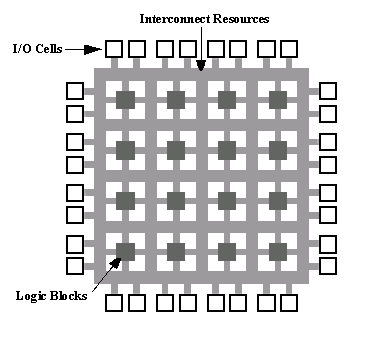
\includegraphics[width = 1\textwidth]{imagenes/arqFPGA.png}
    \caption{\textit{Arquitectura de una FPGA}}\label{arqFPGA}
\end{figure}

Estas FPGAs pueden ser reprogramadas para  algún trabajo específico o para cambiar los requisitos de funcionalidad después de su 
fabricación. Algunas pueden ser programadas una sola vez mientras que otras pueden ser reprogramadas una y otra vez. A estos 
dispositivos que son programados una única vez son referidos como \textbf{OTP} (\textit{one-time programmable}).

\textit{Field Programmable}, se refiere al hecho de que su programación se hace "\textit{en el campo}" a diferencia de otros dispositivos 
que su funcionalidad está programada por el fabricante \cite{maxfield1}.

Hay muchos tipos diferentes de circuitos integrados digitales, entre los que destacamos \textbf{PLDs} (\textit{Programmable Logic Devices}), 
\textbf{ASICs} (\textit{Application-Specific Integrated circuits}), \textbf{ASSPs} (\textit{Application-Specific Standard Parts}) y \textbf{FPGAs}.

Los \textbf{PLDs} son dispositivos con una arquitectura interna predeterminada por el fabricante, creados para ser configurados por 
ingenieros en el campo para realizar diferentes funciones. En comparación a las \textbf{FPGAs}, contiene un número limitado de puertas lógicas 
y las funciones que se suelen implementar son más pequeñas y simples.

Por otro lado los \textbf{ASICs} y los \textbf{ASSPs} contienen cientos de millones de puertas lógicas y se usan para crear grandes y complejas 
funciones. Ambos están basados en los mismos procesos de diseño y tecnologías y pueden ser usados por millones de usuarios y compañias. La 
única diferencia es que un \textbf{ASIC} está diseñado y fabricado para una aplicación en concreto, mientras que un \textbf{ASSP} lo está 
para un dominio de aplicaciones.

Así, las \textbf{FPGAs} se encuentran entre los \textbf{PLDs} y los \textbf{ASICs} porque su funcionalidad puede ser diseñada en el campo como 
los \textbf{PLDs}, pero pueden contener millones de puertas lógicas y ser usadas para implementar funciones complejas que previamente sólo 
podían ser realizadas usando \textbf{ASICs}. 

El coste de un diseño de \textbf{FPGA} es mucho menor que el de uno de un \textbf{ASIC}. Al mismo tiempo, los cambios de diseño implementados 
son más fáciles en \textbf{FPGAs} y el tiempo de comercialización es más rápido \cite{maxfield2}.

Las FPGAs \textbf{SoC}(\textit{System-on-chip}) tienen una gran capacidad de procesamiento para adaptarse a diferentes aplicaciones. Un SoC 
de bajo costo y consumo se puede enfocar en aplicaciones de gran volumen como tarjetas de procesamiento de vídeo o protocolo de puentes. Sin 
embargo, hay otros SoCs que se enfocan en aplicaciones de alto rendimiento en comunicaciones o computación de alto rendimiento.

A mediados del año 1980 llegaron las FPGAs, que eran usadas para implementar lógicas simples, máquinas de estados con una complejidad media 
y tareas de procesamiento de datos. A principios de los 90s, el mercado en el que se vendían se extendió al área de las telecomunicaciones 
debido a que el tamaño y sofisticación de las mismas empezaron a crecer. A finales de los 90s, el uso de las FPGAs en aplicaciones de consumo 
e industriales tuvo un enorme crecimiento.

Las FPGAs a menudo son utilizadas para crear prototipos de diseños ASIC o para tener un plataforma hardware donde verificar la implementación 
física de nuevos algoritmos \cite{maxfield1}. 

Actualmente se pueden encontrar FPGAs de alto rendimiento con millones de puertas. Algunos de estos dispositivos tienen núcleos de 
microprocesador integrados, dispositivos de entrada-salida de alta velocidad y similares. El resultado es que actualmente las FPGAs pueden ser 
usadas para implementar casi cualquier cosa en distintos ámbitos como por ejemplo:

\begin{itemize}
    \item \textbf{Aeroespacial y defensa} 
    \item \textbf{Emulación y Prototipado}
    \item \textbf{Audio} 
    \item \textbf{Automoción} 
    \item \textbf{Broadcast} 
    \item \textbf{Electrónica de consumo} 
    \item \textbf{Centro de procesamiento de datos} 
    \item \textbf{Computación de alto rendimiento} 
    \item \textbf{Industria} 
    \item \textbf{Medicina} 
    \item \textbf{Comunicaciones}
    \item \textbf{Inteligencia Artificial}
    \item \textbf{Procesamiento de imágenes}
    \item \textbf{Seguridad}
\end{itemize}

\section{Niveles de síntesis automática}  

Una de las características principales de un lenguaje de descripción hardware es que a partir de una descripción RTL se puede generar un 
circuito físico. La síntesis es el paso de un nivel de descripción a uno de nivel inferior.

La síntesis física consiste en la ubicación, es decir, decidir dónde colocar todos elementos lógicos, y en el enrutamiento, en el que se 
decide cómo se interconectan los elementos en la FPGA.

La síntesis RT-lógica es un proceso en el se crea un diseño RTL (\textit{Register-Transfer Level}), que es una abstracción del diseño 
en el que se modela el circuito digital, y luego esa representación RTL es convertida a una mezcla de registros y ecuaciones 
booleanas equivalentes. 

La principal diferencia entre síntesis RT y síntesis de alto nivel es que la primera parte de una descripción en la que de forma 
explícita se especifican las operaciones que deben realizarse en cada ciclo de reloj, mientras que la planificación de operaciones 
en ciclos de reloj se realiza de forma automática en la segunda.

La síntesis de alto nivel une hardware y software de manera que los diseñadores hardware pueden trabajar con un alto nivel de abstracción 
y los desarrolladores software pueden acelerar las pas partes computacionalmente complejas de sus algoritmos en una FPGA. 

El uso de una metodología de diseño de síntesis de alto nivel permite desarrollar algoritmos con respecto a la implementación ya que 
consume tiempo de desarrollo, validar el correcto funcionamiento de un diseño de forma más rápida que con lenguajes de descripción 
hardware tradicionales o crear implementaciones hardware de alto rendimiento

\section{Plataformas de desarrollo} 

Actualmente hay muchas empresas que fabrican FPGAs, pero en el top 5 se pueden encontrar \textit{Xilinx}, \textit{Altera}, 
\textit{Lattice Semiconductor}, \textit{Microsemi (antiguo Actel)} y \textit{QuickLogic}. Tanto Xilinx como Altera ocupan un 89\% 
del mercado, siendo Xilinx el líder desde hace muchos años. Xilinx tiene bastante variedad de FPGAs en cuanto a coste y rendimiento. 
Actualmente, la serie \textit{Virtex} y la serie \textit{Zynq-7000} de SoC ocupan el mercado de gama alta, la serie \textit{Kintex} 
de gama media y la serie \textit{Artix} de gama baja junto con la \textit{Spartan} que ha sido retirada del mercado.

La serie \textit{Virtex} integra lógica \textbf{FIFO} y \textbf{ECC}, bloques \textbf{Ethernet MAC}, bloques \textbf{DSP} (\textit{Procesador 
de señales digitales}), controladores \textbf{PCI-Express}. Además incluye hardware embebido con una función fija para funciones que se 
usan comúnmente como multiplicadores o memoria. 

La serie \textit{Kintex} se caracteriza por consumir menos energía que la serie anterior, incluyendo alto rendimiento y elementos necesarios 
para aplicaciones que tengan mucho volumen.

La serie \textit{Artix} se basa en la arquitectura unificada de la serie \textit{Virtex}. Esta serie está diseñada para aplicaciones con 
rendimiento de bajo consumo. 

Dependendiendo de la síntesis que queramos realizar podemos encontrar distintos software:

\begin{itemize}
    \item \textbf{Herramientas de síntesis RT-lógica}:
        \begin{itemize}
            \item \textit{Synplify Pro}, \textit{Synplify Premier} (\textit{Synopsis})
            \item \textit{Precision RTL Plus}, \textit{LeonardoSpectrum} (\textit{Mentor Graphics})
            \item \textit{Quartus} (\textit{Altera})
            \item \textit{Vivado} (\textit{Xilinx})
        \end{itemize}
    \item \textbf{Herramientas de síntesis de alto nivel}:
        \begin{itemize}
            \item \textit{Synphony C Compiler} (\textit{Synphony})
            \item \textit{Impulse coDeveloper} (\textit{Impulse C})
            \item \textit{Vivado High Level Synthesis} (\textit{Xilinx})
            \item \textit{SDSoc} (\textit{Xilinx})
            \item \textit{SDAccel} (\textit{Xilinx})
            \item \textit{Intel SDK for OpenCL} (\textit{Intel Altera})
            \item \textit{Intel HLS Compiler} (\textit{Intel Altera})
        \end{itemize}
\end{itemize}

La última herramienta comercializada por Xilinx, \textit{Vitis} es un entorno de desarrollo de aplicaciones que sustituye a las herramientas 
\textit{SDSoc} y \textit{SDAccel} que permite utilizar tanto FPGAs en tarjetas aceleradoras on premise y en la nube, como FPGAs con procesadores 
empotrados. Incorpora una herramienta de síntesis de alto nivel (\textbf{Vitis HLS}) que pretende reducir las diferencias entre escribir 
funciones para su ejecución software o para su implementación hardware. Y se dispone incluso de bibliotecas con funciones prediseñadas 
para diferentes dominios de aplicación (inteligencia artificial, visión, etc.).

Las plataformas de desarrollo con propósito académico que comercializa Xilinx son \cite{students}:

\begin{itemize}
    \item \textbf{7-series} - \textit{Spartan-7}, \textit{Artix-7}, \textit{Kintex-7}, \textit{Virtex-7}
    \item \textbf{Zynq} - \textit{ZYBO}, \textit{ZYBO Z7}, \textit{ZedBoard}
    \item \textbf{Spartan} - \textit{Spartan-6}, \textit{Spartan-3E}
    \item \textbf{Virtex} - \textit{Virtex-6}, \textit{Virtex-5}, \textit{Virtex-4}, \textit{Virtex-2P}
\end{itemize}


\section{Estructura de la memoria} 
 
 
 

\chapter{Objetivos del trabajo}

El principal objetivo de este TFG es el conocimiento de una plataforma de carácter didáctico orientada a FPGAs de la familia Zynq de Xilinx para la 
realización de diferentes ejercicios prácticos útiles en el aprendizaje en asignaturas relacionadas con el diseño de sistemas 
basados en dispositivos hardware reconfigurables.

La empresa Xilinx es una empresa líder en el desarrollo de herramientas no sólo a nivel de síntesis RT-lógica, sino 
también de síntesis de alto nivel y particularmente para co-diseño HW/SW de sistemas empotrados en FPGAs basado en aplicaciones y 
descripciones tipo C/C++. Sus herramimentas se han utilizado en asignaturas de perfil más avanzado y resulta conveniente la 
migración a este tipo de plataformas de las prácticas que se realizan en otras asignaturas de perfil más básico, con intención de 
favorecer al estudio con una misma plataforma basada en la herramienta Vivado y una tarjeta de desarrollo basada en
FPGAs Zynq.
 
Se toma como referencia la asignatura "Desarrollo de hardware digital" de la especialidad de Ingeniería de Computadores que pertenece al 
grado de Informática, cuyos contenidos se corresponden fundamentalmente con el aprendizaje de la metodología de diseño de sistemas basados en FPGAs con herramientas de síntesis 
automática y verificación a partir de descripciones VHDL en el nivel RT, para el análisis y diseño de módulos hardware específicos, tales 
como procesadores específicos, memorias, y módulos de interfaz y comunicaciones.

Y por último se establecen siguientes objetivos:
\begin{enumerate}
    \item Estudio y descripción de cómo se realiza en Vivado la metodología propia de flujo de diseño con FPGAs a partir de descripciones RT en VHDL.
    \item Descripción módulos de especial interés en la plataforma para la realización de prácticas (procesador, memoria, interfaz VGA, generación de reloj).
    \item Realización de dos casos prácticos planteados en la asignatura para comprobar la utilidad y el correcto funcionamiento de los módulos que en este 
    momento integran la plataforma junto con la tarjeta Zybo y la herramienta Vivado.
\end{enumerate}

\input{capitulos/05_Resolución}

\chapter{Conclusiones y vías futuras}



\clearpage
\nocite{*}
\bibliographystyle{plain}
\bibliography{bibliografia/bibliografia}

%Se incluirá tanto las fuentes primarias como todas aquellas cuyo peso haya sido menor en la realización del trabajo. Un breve comentario de las referencias es conveniente, que puede ser individualizado, por grupos de referencias o global.
%En caso de incluir URLs de páginas web (se recomienda no abusar de ellas), éstas deben ser acompañadas de título, autor, fecha de último acceso, entre otros datos relevantes.

\end{document}
